\section{Signal mass spectrum shape}
\label{sec:signal_mass_spectrum_shape}

Resonances coupling weakly to the Standard Model are by definition
narrow, so their lineshapes are dominated by detector resolution and
final state radiation of a photon from one of the muons. The Standard
Model provides four resonances in our mass range of interest,
$\omega$, $\phi$, $J/\psi$, and $\psi'$, which we use to calibrate the
signal lineshapes.  These resonances are typically produced with low
momentum, so we additionally simulate low and high momentum resonances
with a dimuon-gun Monte Carlo. We study the resolution of each of these
resonances and find a good agreement with the expectation as shown in
Figure~\ref{fig:resolution} summarizes the results of these fits in
bins of dimuon $p_T$, mass, and $\eta$ coverage.  The results of the
resonance data fits are overlaid for comparison.  The core Gaussian
dependence on $p_T$ and $\eta$ are weak, but higher momenta and larger
$\eta$ coverage yield slightly wider core resolutions.  The
double-Gaussian part of the distribution, however, grows strongly as a
function of mass for high-$p_T$ dimuons in the endcap.

For more sensitivity to extremes in $p_T$ and $\eta$, distributions of
reconstructed mass minus generator-level mass from the dimuon gun
Monte Carlo were fitted to double Gaussians.  Backgrounds ($p_0$ and
$p_1$) and final-state radiation ($\alpha$) were not included in the
fit because the effects were not simulated.


\begin{figure}
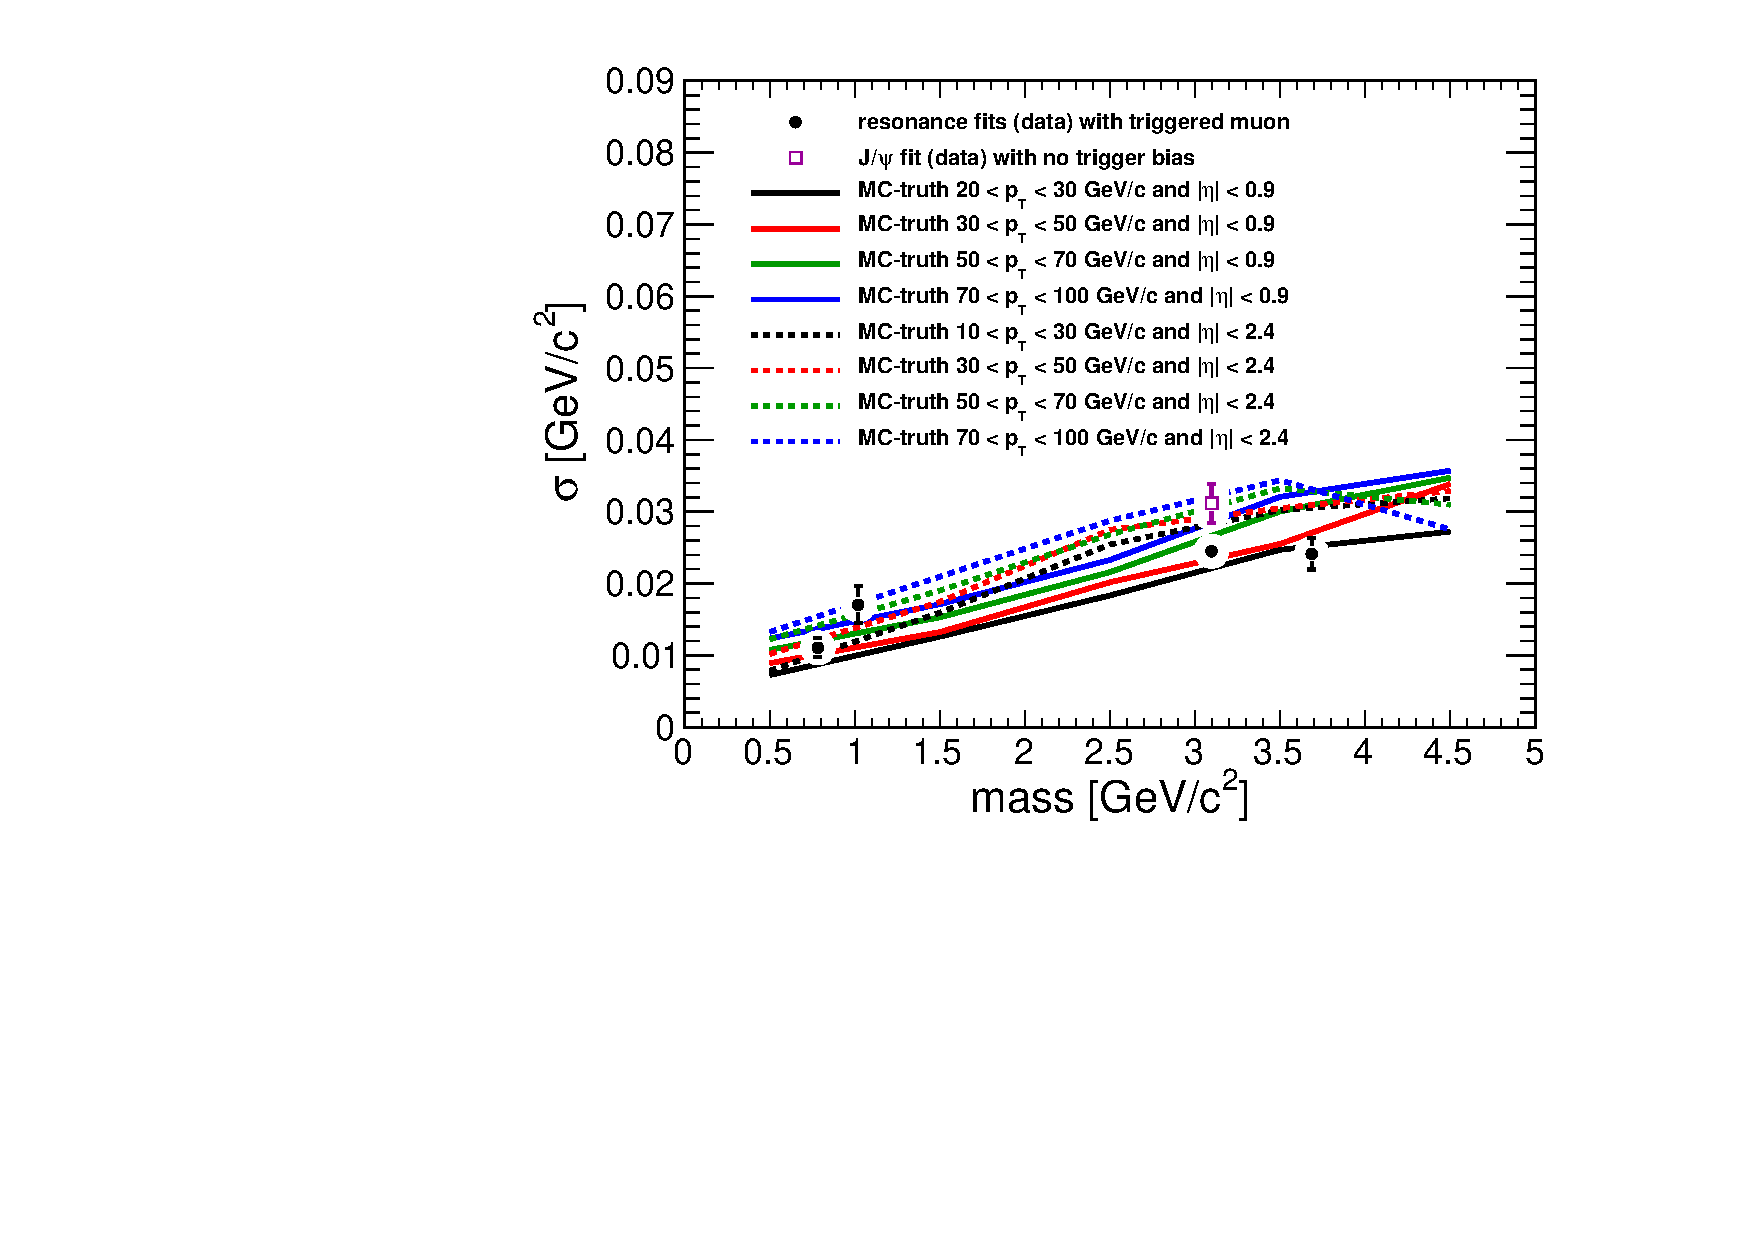
\includegraphics[width=0.5\linewidth]{PLOTS/resolution.pdf}
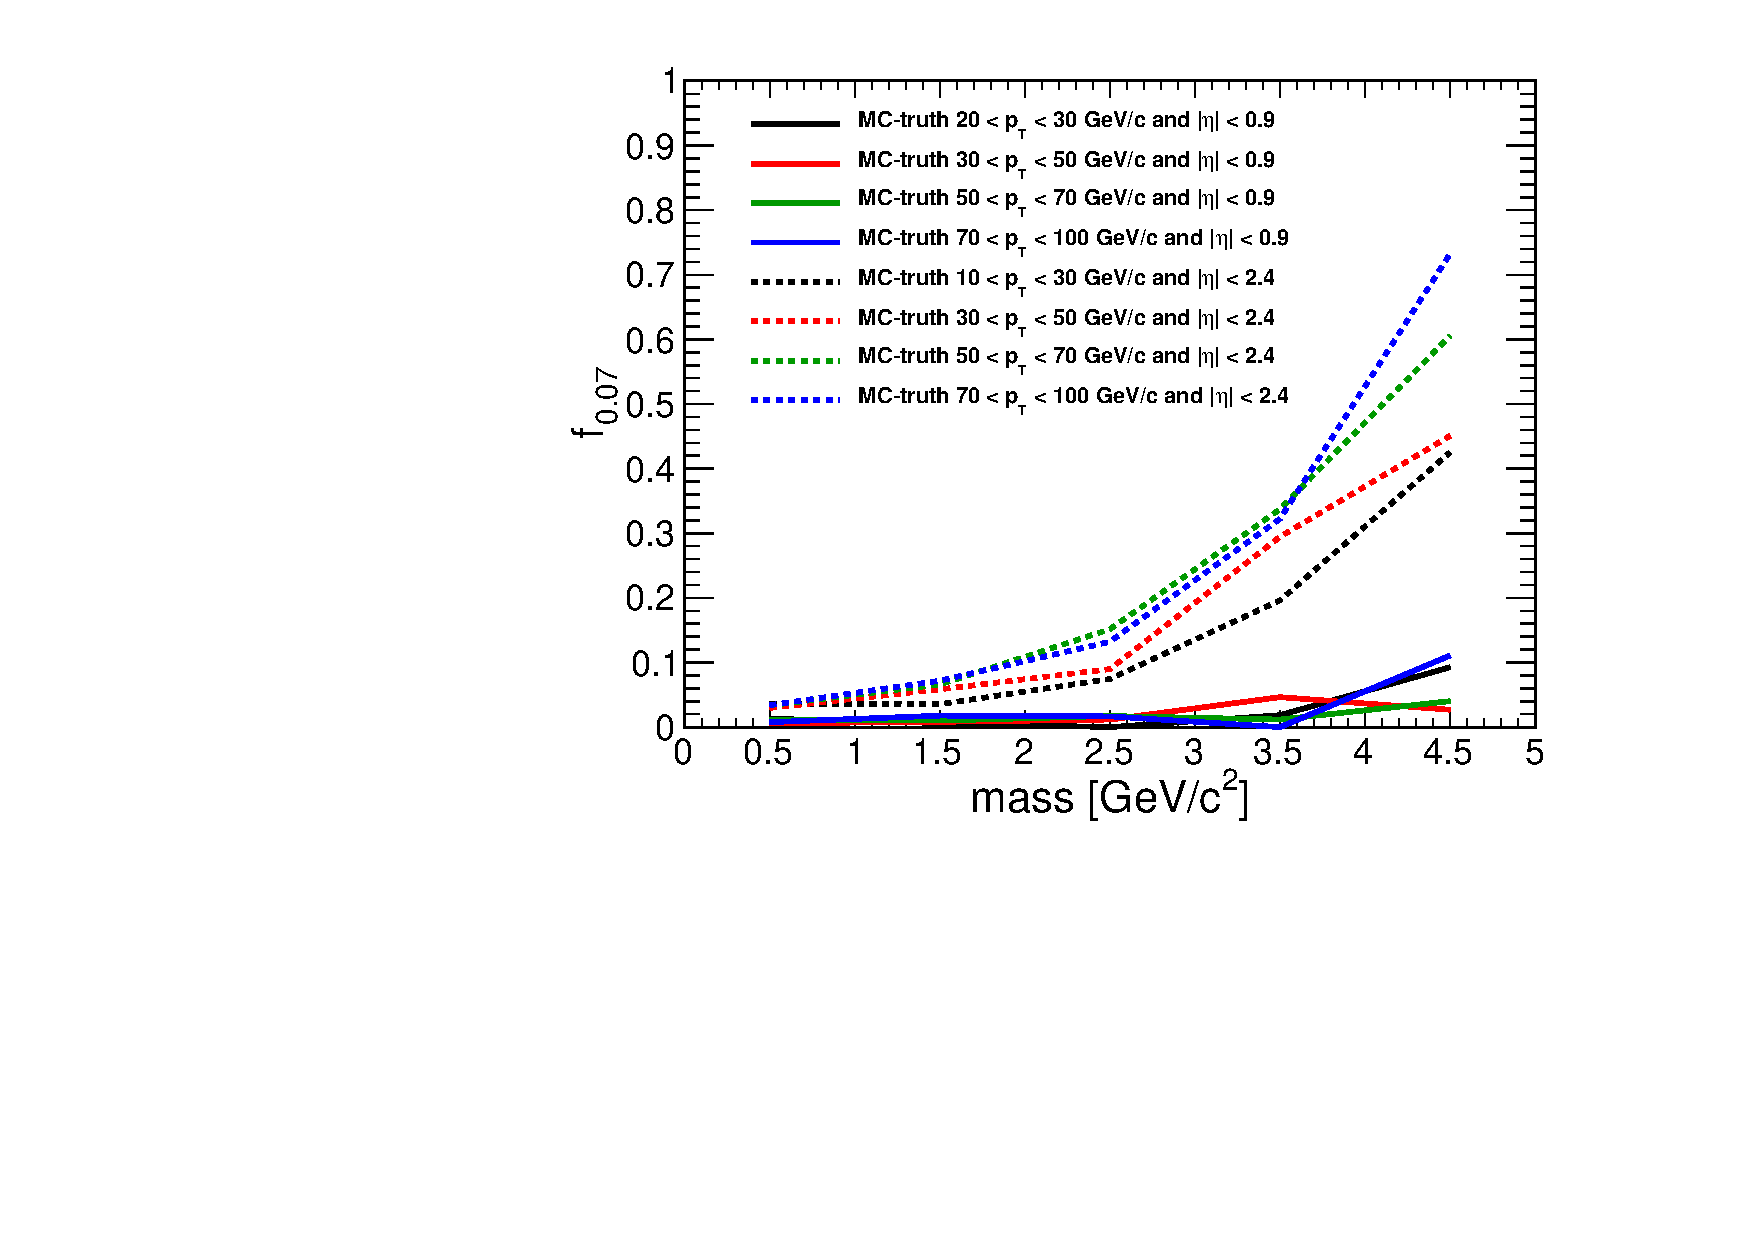
\includegraphics[width=0.5\linewidth]{PLOTS/resolution_f007.pdf}

\caption{Left: resolution as a function of mass for simulated muons
  (lines) and real resonances (points).  Right: the double-Gaussian
  parameter $f_{0.07}$ for simulated muons. \label{fig:resolution}}
\end{figure}
